%%%%%%%%%%%%%%%%%%%%%%%%%%%%%%%%%%%%%%%%%
% University Assignment Title Page 
% LaTeX Template
% Version 1.0 (27/12/12)
%
% This template has been downloaded from:
% http://www.LaTeXTemplates.com
%
% Original author:
% WikiBooks (http://en.wikibooks.org/wiki/LaTeX/Title_Creation)
%
% License:
% CC BY-NC-SA 3.0 (http://creativecommons.org/licenses/by-nc-sa/3.0/)
% 
% Instructions for using this template:
% This title page is capable of being compiled as is. This is not useful for 
% including it in another document. To do this, you have two options: 
%
% 1) Copy/paste everything between \begin{document} and \end{document} 
% starting at \begin{titlepage} and paste this into another LaTeX file where you 
% want your title page.
% OR
% 2) Remove everything outside the \begin{titlepage} and \end{titlepage} and 
% move this file to the same directory as the LaTeX file you wish to add it to. 
% Then add \input{./title_page_1.tex} to your LaTeX file where you want your
% title page.
%
%%%%%%%%%%%%%%%%%%%%%%%%%%%%%%%%%%%%%%%%%
%\title{Title page with logo}
%----------------------------------------------------------------------------------------
%	PACKAGES AND OTHER DOCUMENT CONFIGURATIONS
%----------------------------------------------------------------------------------------

\documentclass[12pt]{article}
\usepackage[french]{babel}
\usepackage[utf8x]{inputenc}
\usepackage{amsmath}
\usepackage{graphicx}
\usepackage[colorinlistoftodos]{todonotes}
\usepackage{listings}
\usepackage{float}
\usepackage[justification=centering]{caption}
\usepackage[toc,page]{appendix}
\renewcommand{\appendixtocname}{Annexes} 
\renewcommand{\appendixpagename}{Annexes} 
\begin{document}

\begin{titlepage}

\newcommand{\HRule}{\rule{\linewidth}{0.5mm}} % Defines a new command for the horizontal lines, change thickness here

\center % Center everything on the page
 
%----------------------------------------------------------------------------------------
%	HEADING SECTIONS
%----------------------------------------------------------------------------------------

\textsc{\LARGE Université Pierre et Marie Curie}\\[1.5cm] % Name of your university/college
\textsc{\Large Projet SAR}\\[0.5cm] % Major heading such as course name
\textsc{\large }\\[0.5cm] % Minor heading such as course title

%----------------------------------------------------------------------------------------
%	TITLE SECTION
%----------------------------------------------------------------------------------------

\HRule \\[0.4cm]
{ \huge \bfseries Application embarquée sur carte pour l'automobile}\\[0.4cm] % Title of your document
\HRule \\[1.5cm]
 
%----------------------------------------------------------------------------------------
%	AUTHOR SECTION
%----------------------------------------------------------------------------------------

\begin{minipage}{0.4\textwidth}
\begin{flushleft} \large
\emph{Auteurs:}\\
Maxime \textsc{Bittan}\\
Redha \textsc{Gouicem}\\
Ilyas \textsc{Toumlilt} 
\end{flushleft}
\end{minipage}
~
\begin{minipage}{0.4\textwidth}
\begin{flushright} \large
\emph{Encadrants:} \\
Antoine \textsc{Blin}\\
Gilles \textsc{Muller}\\
Julien \textsc{Sopena}
\end{flushright}
\end{minipage}\\[2cm]

% If you don't want a supervisor, uncomment the two lines below and remove the section above
%\Large \emph{Author:}\\
%John \textsc{Smith}\\[3cm] % Your name

%----------------------------------------------------------------------------------------
%	DATE SECTION
%----------------------------------------------------------------------------------------

{\large \today}\\[2cm] % Date, change the \today to a set date if you want to be precise

%----------------------------------------------------------------------------------------
%	LOGO SECTION
%----------------------------------------------------------------------------------------


\includegraphics[scale=0.1]{include/logo_upmc.png}  % Include a department/university logo - this will require the graphicx package
\hspace{1cm}

\includegraphics[scale=0.15]{include/logo_lip6.png} % Include a department/university logo - this will require the graphicx package
\hspace{1cm}

\includegraphics[scale=0.06]{include/logo_renault.png}\\
%----------------------------------------------------------------------------------------

\vfill % Fill the rest of the page with whitespace

\end{titlepage}

%-------------------------------------------------------------------------------
% BODY
%-------------------------------------------------------------------------------

\tableofcontents

\section*{Introduction}

Dans la plupart des domaines des systèmes embarqués, comme l'industrie du transport, il est nécessaire d'exécuter les applications à différents niveaux de criticité. Certaines applications demandent beaucoup de contraintes temps-réel, alors que d'autres se contentent d'accès ordonnancé aux ressources ( CPU, Mémoire ).\\
\\
Ce sujet s'intègre dans le cadre d'une collaboration avec Renault portant sur l'exécution de tâches à criticité mixte sur un multi-coeur.\\
Le but de ce PSAR est de porter une application sur une carte industrielle.\\
La carte en question est une Freescale SABRE Lite Board, qui nous offre suffisamment de puissance CPU pour exécuter plusieurs applications. Elle embarque un système multi-cœur ( Linux 3.0.35 ) , où dans notre approche, un coeur exécute l'application temps réel, tandis que les trois autres exécutent notre application.\\
\\
Le premier objectif de ce PSAR étant donc de trouver une application satisfaisant les contraintes de notre approche, à savoir, la génération de flux de traffic de données important sur le bus, et l'exécution en multi-coeur.\\
Le choix c'est donc porté sur une application de mapping, GPS.\\
\\
Une deuxième étape consiste à porter notre application sur la carte, après configuration de cette dernière, ce qui posera donc à nouveau des contraintes de compatibilité et de nombre de dépendances, et rajoutera encore un nouveau critère de sélection d'application : le moins de dépendances, pour moins de complexité de portage.\\
\\
Une fois l'application portée, on en fera le profil mémoire, à l'aide d'un outil développé dans l'équipe. Cet outil détermine le profil d'utilisation de la bande passante mémoire par une application temps réel, et nous permettra d'étudier  l'impact de notre application sur la tâche temps réel s'exécutant sur le coeur dédié.\\
\\

\clearpage


\section{La carte SABRE Lite}

\subsection{Caractéristiques techniques}

\subsubsection{Architecture interne}
La carte SABRE Lite\cite{_i.mx_2014} embarque un processeur i.MX 6, basé sur le processeur ARM
Cortex A9 MPCore. Il s'agit d'un processeur quad-core cadencée à 1 GHz, 
disposant de caches L1 de 32 Ko ainsi que d'un cache L2 de 1 Mo partagé pour les
quatre coeurs. La carte dispose également de 1 Go de mémoire vive (DDR3). Le
contrôleur mémoire contient plusieurs compteurs permettant la mesure de 
l'activité mémoire qui seront utilisés dans la phase de profilage détaillée dans
la suite de ce rapport. Une puce de mémoire flash SPI de 2 Mo contenant un code
de boot est aussi présente.

\subsubsection{Stockage}
Le système ne dispose pas de stockage de masse interne intégré mais de ports
permettant l'ajout de périphériques de stockage :
\begin{itemize}
\renewcommand{\labelitemi}{$\bullet$}
\item un port SATA pour connecter un disque dur ou un SSD,
\item deux ports USB 2.0,
\item un port microUSB 2.0 supportant la norme OTG, afin de permettre au 
  périphérique de commander les échanges vers la carte,
\item un port SD et un port microSD.
\end{itemize}

\subsubsection{Autres connectiques}
La carte dispose également d'un port Ethernet pour se connecter au réseau, ainsi
que d'un port UART, permettant une liaison série avec un ordinateur. Cette
liaison série sera notamment utilisée lors de la configuration de la carte. La
carte embarque également les ports suivants :
\begin{itemize}
\renewcommand{\labelitemi}{$\bullet$}
\item HDMI
\item microphone et casque
\item GPIO/I2C
\item PCIe
\item LVDS (Low-Voltage Differential Signaling)
\item caméra
\end{itemize}

\subsection{Image système}
Afin de rendre la carte utilisable, il est bien entendu nécessaire d'y installer
un système d'exploitation. Il est possible de booter la carte de deux manières:
\begin{itemize}
\renewcommand{\labelitemi}{$\bullet$}
\item via le port microUSB OTG,
\item via la mémoire flash interne
\end{itemize}
Le mode de boot est contrôlé par un interrupteur sur la carte. Dans notre cas,
nous allons utiliser le code de boot préchargé dans la mémoire flash interne
pour ensuite charger l'image présente sur une carte microSD et démarrer sur
cette dernière.

\subsubsection{Construction de l'image}
Afin de construire l'image système pour la carte SABRE Lite, nous allons
utiliser la suite d'outils du projet Yocto\cite{hallinan_create_2015}. Il s'agit
d'un projet géré par la Linux Foundation et plusieurs grandes entreprises du
monde de l'embarqué (Intel, Texas Instruments, Huawei, ...). Cette suite permet
notamment la construction d'images Linux personnalisées pour systèmes embarqués.
La construction se fait par couches (\texttt{layers}), chacune représentant un
ensemble logique de recettes (\texttt{recipes}). Une recette est une suite
d'instructions détaillant des étapes de construction (dépendance à d'autres
recettes, origine des sources, paquets à installer, ...).

\paragraph{} Après avoir concocté les couches et les recettes nécessaires à la
construction de l'image système (l'ajout d'un client \texttt{ssh} à une image
minimale dans notre cas), l'outil \texttt{bitbake}\cite{purdie_bitbake_????}
de la suite Yocto exécute toutes les recettes. Ce dernier construit entièrement
l'image pour le système ciblé, notamment en téléchargeant les sources de tous
les paquets et en les recompilant un à un. Des partitions (image kernel
\texttt{uImage}, rootfs), ainsi qu'une image pour carte SD contenant ces
dernières, sont alors générées.

\subsubsection{Déploiement de l'image}
L'image se déploit très simplement sur une carte SD, soit en copiant via un
outil tel que \texttt{dd} l'image pour carte SD générée, soit en partitionnant
la carte SD (Figure \ref{partSD}) et en copiant les partitions générée une à une
\cite{angolini_yocto_2014}.

\begin{figure}
  \centering
  \begin{tabular}{|c|c|c|c|}
    4 Mio & 8 Mio & ROOTFS\_SIZE & 4 Mio \\
    \hline
    réservé au bootloader & kernel & rootfs & non \\
    (non partitionné) & (uImage) & & partitionné \\
  \end{tabular}
  \caption{Partitionnement de la carte SD}
  \label{partSD}
\end{figure}

\paragraph{} Maintenant que la carte SD est prête, il faut configurer notre
SABRE Lite afin de booter sur celle-ci. Pour cela, nous allons tout d'abord
démarrer sur le mémoire flash SPI qui contient un code de boot
(\texttt{U-Boot}\cite{denk_denx_2015}) préchargé. Sur cet environnement de
boot, il est possible de gérer les périphériques, de configurer la séquence de
boot, etc... \\
Dans notre cas, nous avons seulement :
\begin{itemize}
\renewcommand{\labelitemi}{$\bullet$}
\item sélectionné le port microSD, 
\item configuré les arguments de boot du kernel Linux (nom et débit de la console,
  chemin vers le \textit{rootfs}, \texttt{rootwait} pour que le kernel attende
  la détection de la carte SD),
\item chargé l'image kernel (\texttt{uImage}) en mémoire,
\item et enfin booté à l'adresse de l'image kernel.
\end{itemize}
(Figure \ref{ubootcmds})

\begin{figure}[H]
  \centering
  \begin{lstlisting}[language=bash, frame=single, basicstyle=\scriptsize]
    mmc dev 1
    fatload mmc 1:1 0x10800000 uImage
    setenv bootargs console=ttymxc1,115200 rootwait root=/dev/mmcblk0p2
    bootm
  \end{lstlisting}
  \caption{Commandes de configuration du U-Boot}
  \label{ubootcmds}
\end{figure}

\paragraph{}
Les différents essais de déploiement d'images que nous avions nous mêmes créées
ont systématiquement échoué lors du boot, la carte se bloquant lors du boot
du kernel, après avoir été chargé en mémoire. Faute de temps, nous n'avons pu
réoudre ce problème et nous sommes donc tournés vers une image déjà créée et
fonctionnelle, afin de nous concentrer sur la suite du projet, à savoir le
portage de l'application ainsi que le profilage sur la carte.


P2 empty file


\section{Profilage}

Dans cette partie, nous allons mesurer et essayer d'interpréter l'impact de 
l'exécution d'une tâche \textit{best effort} sur une application temps-réel.
La tâche \textit{best effort} sera l'application Routino dans ses versions
monothread et multithread, et les tâches temps-réel seront les applications de
la suite de benchmark MiBench\cite{guthaus_mibench:_2001}. Ces mesures seront
séparées en deux parties : une analyse de l'impact sur le temps d'exécution
suivie d'une analyse de l'impact sur la bande passante. Nous essayerons ensuite
de corréler ces deux analyses.

\subsection{Analyse temporelle}
Afin d'analyser l'impact sur le temps d'exécution de la tâche temps-réel, nous
avons d'abord considérer chaque application temps-réel individuellement, puis
l'ensemble des applications comme une unique tâche, afin d'avoir un échantillon
plus important. Pour ces deux jeux de mesures, nous avons mesuré la durée 
d'exécution de la tâche temps-réel s'exécutant en isolation sur le système,
puis en concurrence avec trois instances de Routino monothread occupant
chacune un coeur, et enfin en concurrence avec un Routino multithread utilisant
trois threads effectuant les calculs. Nous calculons ensuite le surcoût en
termes de temps d'exécution par rapport à l'exécution seule de la tâche
temps-réel (Table \ref{timebench}). Il faut noter que
dans le cas où les tâches temps-réel sont analysées individuellement, les 
instances de Routinos concurrentes sont lancées en même temps que la tâche 
temps-réel et stoppées dès la fin de cette dernière. Les mesures sont ainsi
comparables, puisque chaque tâche aura été confrontée à une partie similaire 
de l'exécution de Routino.

\begin{table}[h]
\centering
\begin{tabular}{l|c|c|c|c|c}
Tâche & Temps moyen & \multicolumn{2}{c|}{Avec 3 Routinos} & 
\multicolumn{2}{c}{Avec Routino MT} \\
 & seule & Temps & Surcoût & Temps & Surcoût\\
\hline
susan\_c & 25.1 & 26.5 & 5.75\%  & 28.3 & 12.87\%\\
susan\_e & 57.2 & 58.2 & 1.60\%  & 59.4 & 3.85\%\\
fft      & 3.1  & 3.6  & 15.51\% & 3.7  & 18.64\%\\
fft\_i   & 9.3  & 10.7 & 14.72\% & 11.2 & 20.75\%\\
aes\_e   & 42.2 & 43.2 & 2.18\%  & 44.1 & 4.31\%\\
aes\_d   & 41.7 & 43.3 & 3.71\%  & 43.3 & 3.71\%\\
qsort    & 27.5 & 30.7 & 11.87\% & 32.2 & 17.14\%\\
patricia & 58.2 & 64.3 & 10.54\% & 64.5 & 10.87\%\\
\hline
Toutes   & 264.8 & 278.4 & 5.13\%  & 283.8 & 7.16\%\\
\end{tabular}
\caption{Temps d'exécution en isolation puis en concurrence (en ms) et surcoût}
\label{timebench}
\end{table}

\paragraph{}
On remarque que dans plus de la moitié des cas, le surcoût dépasse les 10\%, ce
qui pose problème pour des tâches supposées s'exécuter en temps-réel. La tâche
\textit{best effort}, à savoir Routino, a donc un impact conséquent sur le bon
fonctionnement du système. De manière plus concrète, cela signifie que le 
calcul d'itinéraire du GPS pourrait retarder la prise d'information du radar
de régulation de distance, et causer un danger pour les passagers du véhicule.

\subsection{Analyse de bande passante}
Nous allons maintenant mesurer la bande passante utilisée lors de ces
exécutions, en reprenant le même protocole que pour les mesures de temps. Les
résultats obtenus (Figure \ref{bandwidth}) seront comparées aux
mesures réalisées par Blin et al. \cite{blin_protecting_2015} et qui ont
conduit à ce projet (approximations en Table \ref{measures}).

\begin{figure}
\centering
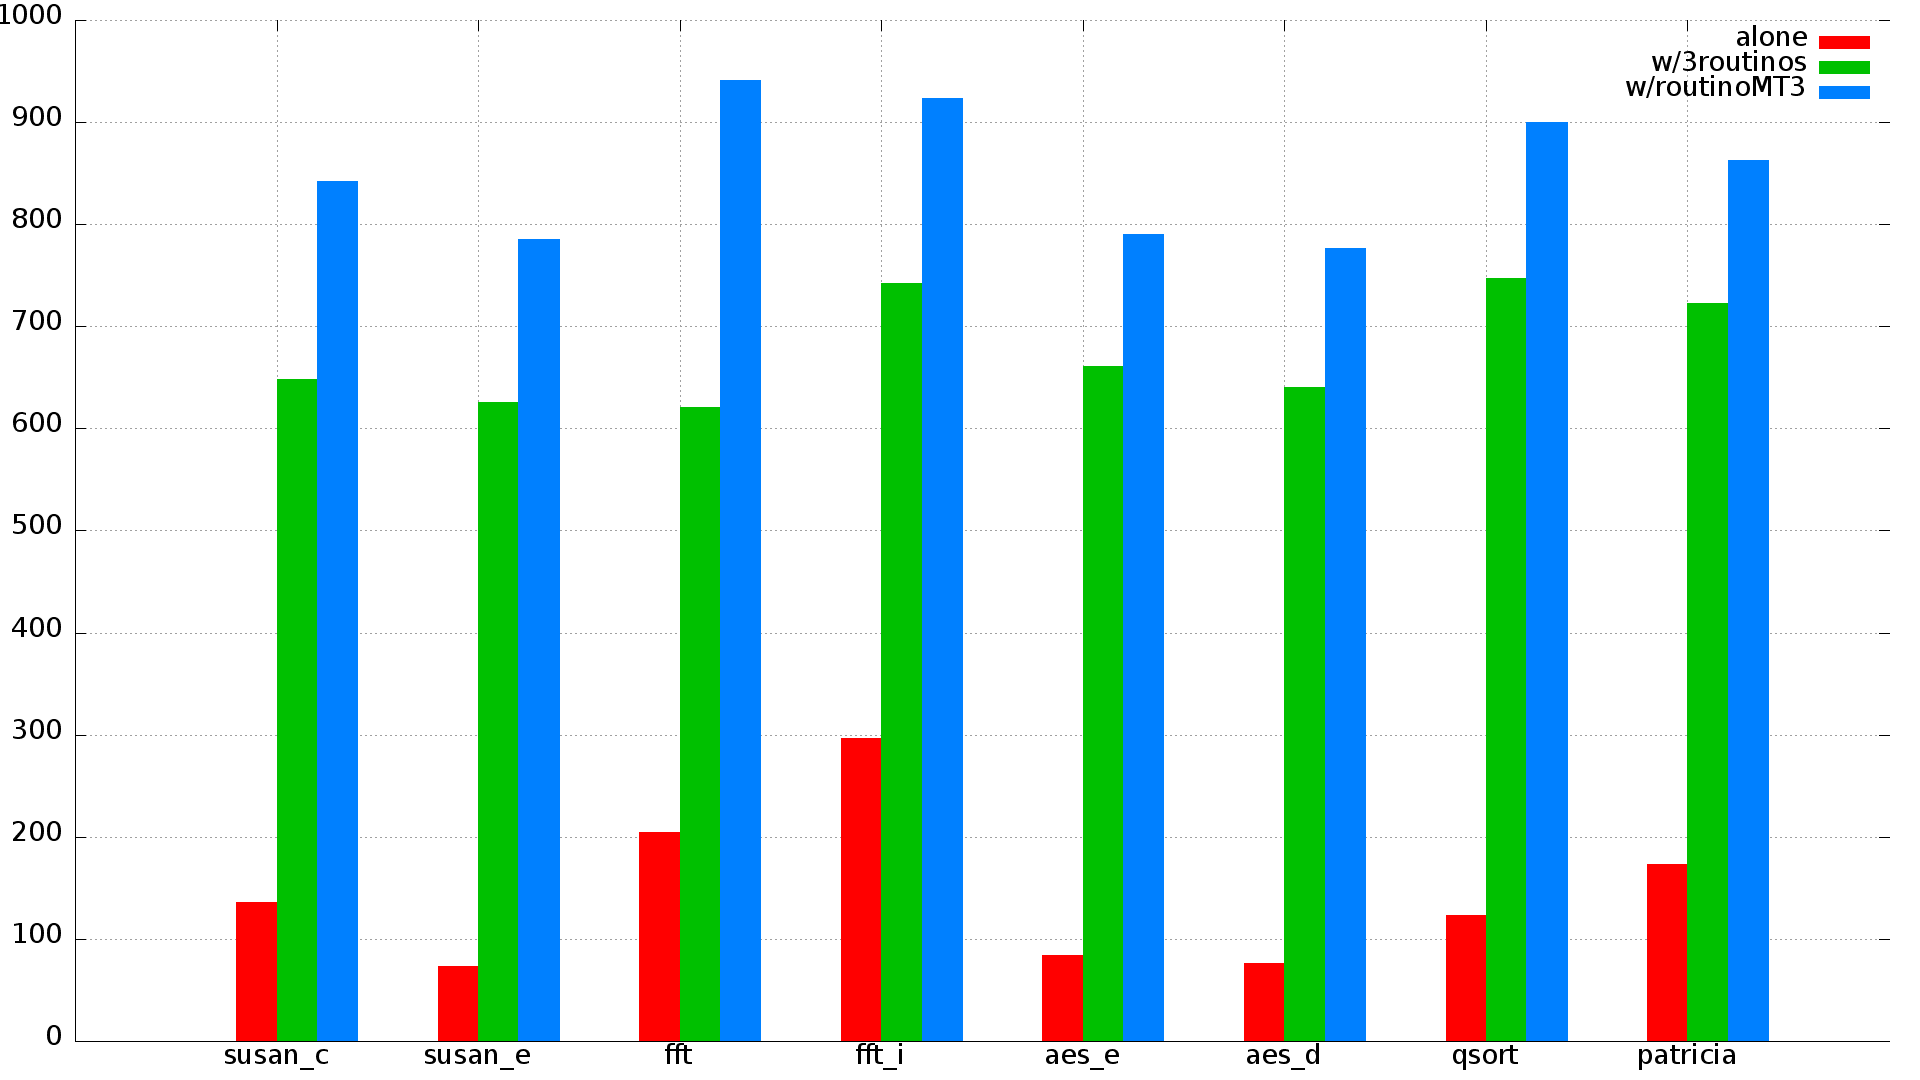
\includegraphics[scale=0.285]{include/bandwidth.png}
\caption{Utilisation moyenne de la bande passante lors des exécutions du
 MiBench (en Mo/s)}
\label{bandwidth}
\end{figure}

\begin{table}[H]
\centering
\begin{tabular}{l|c}
Tâche & Besoins bande passante (Mo/s)\\
\hline
susan\_c & 750\\
susan\_e & 600\\
fft      & 200\\
fft\_i   & 250\\
aes\_e   & 450\\
aes\_d   & 350\\
qsort    & 600\\
patricia & 500\\
\end{tabular}
\caption{Profils mémoire des tâches temps-réel}
\label{measures}
\end{table}

\paragraph{}
En nous basant sur les profils mémoire (Table \ref{measures}), les
mesures d'utilisation de bande passante (Figure \ref{bandwidth}) et sur la
caractérisation du système réalisée par Blin et al.\cite{blin_protecting_2015},
nous dressons la table \ref{carac} donnant les surcoûts que nous devrions
observer, ainsi que les surcoûts observés pour le Routino multithread.

\begin{table}[H]
\centering
\begin{tabular}{l|c|c||c}
Tâche & Caractérisation & Mesures & \'Ecart\\
\hline
susan\_c & ~20\% & 12.87\% & 7.13\%\\
susan\_e & ~5\%  & 3.85\%  & 1.15\%\\
fft      & ~2\%  & 18.64\% & 16.64\%\\
fft\_i   & ~2\%  & 20.75\% & 18.75\%\\
aes\_e   & ~5\%  & 4.31\%  & 0.69\%\\
aes\_d   & ~2.5\%& 3.71\%  & 1.21\%\\
qsort    & ~20\% & 17.14\% & 2.86\%\\
patricia & ~10\% & 10.87\% & 0.87\%\\
\end{tabular}
\caption{Surcoûts selon caractérisation du système et surcoûts mesurés avec
Routino multithread}
\label{carac}
\end{table}

\paragraph{}
On remarque que dans la majorité des cas, nos mesures sont cohérentes avec la
caractérisation du système. Seules \texttt{fft} et \texttt{fft\_i} ont des
écarts conséquents (plus de 15\%). Cela est probablement dû à la courte durée
de ces tâches. En effet, leur exécution coïncide avec la période où
Routino charge en mémoire de forts volumes de données (chargement de la carte)
uniquement. Elles se terminent sûrement avant que Routino ne commence à 
réellement calculer l'itinéraire. L'impact de la tâche \textit{best effort} est
donc important sur la tâche temps-réel.


\section*{Conclusion}
Conclusion empty file


\begin{appendices}
  \section{Utilisation de Routino}
  \subsection{toto}
\end{appendices}

\clearpage

\bibliographystyle{plain}
\bibliography{bibliography}

\end{document}
